\subsection{Language Concepts}\label{sec:langconcepts}

\newcommand{\fcontrolflow}{\f{ControlFlow}}
\newcommand{\fmodularity}{\f{Modularity}}
\newcommand{\fdatatypes}{\f{DataTypes}}
\newcommand{\fevents}{\f{EventSupport}}
\newcommand{\freadsensor}{\f{ReadSensor}}
\newcommand{\fcontrolflowparadigm}{\f{ControlFlowParadigm}}
\newcommand{\factions}{\f{Actions}}
\newcommand{\fexceptions}{\f{ExceptionHandling}}
\newcommand{\ffileaccess}{\f{FileAccess}}
\newcommand{\ffunctionlib}{\f{FunctionLibrary}}
\newcommand{\fmultithread}{\f{Multithreading}}

%In Language concepts feature, figure \ref{sec:langconcepts}, we identified eleven sub-features, from which three are considered mandatory: control flow, actions and control flow paradigm . 
%We did not find a situation where all the optional features do not exist in a particular language.

We found a range of different concepts offered by the languages for specifying missions. We consider a concept a distinct element of the abstract syntax of the language. We focus on concepts that are recognizable via the notation (concrete syntax), since many of our environments are not open-source, preventing a look at the exact implementation of the language's abstract syntaxes. End-users observe these concepts via the language's notation and utilize them via the respective projectional editor, except for the textual additional languages provided by some environments. As shown in \figref{fig:langconcepts}, we classified the concepts we found into the features: \fcontrolflowparadigm, \fcontrolflow, \fmodularity, \fdatatypes, \fevents, \freadsensor, \factions, \fexceptions, \ffileaccess, \ffunctionlib, and \fmultithread, as detailed below.

%Language concepts is a sub-feature of languages that %is treated separately because it 
%highlights the concepts that determine the expressiveness of the language while specifying missions. Sub-features of the language concepts include: control flow, modularity of the language, variable data types supported, event support ability, the types of sensor data that can be read, control flow paradigm, actions the robots can perform, exception handling, file access feature, function libraries, and multithreading support.

%The expressive power of the environments is determined by the language concepts that are salient to the end-user. As shown in \figref{fig:langconcepts}, we categorized these concepts into control flow, modularity concepts, variable data types, event support, read sensor, control flow paradigms, actions, exception handling, file access, function  library, and multi-threading.  

\begin{figure}[t]
     \centering
    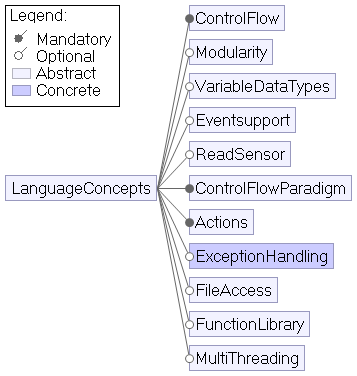
\includegraphics[width=.6\columnwidth]{LanguageConcepts.png}
      \caption{Language Concepts%\tb{change VariableDataTypes to DataTypes}
      }
      \label{fig:langconcepts}
			\vspace{-.4cm}
   \end{figure}

\parhead{\fcontrolflowparadigm.} One of the core distinguishing characteristics is the kind of control-flow paradigm supported by the languages, which determines how missions are executed. We found three major kinds: 
\begin{itemize}
	\item the imperative paradigm;
	\item the reactive paradigm;
	\item the goal-based paradigm.
\end{itemize}

The former two are relatively low-level; none of our environments supports a purely goal-based paradigm, where the goal to be achieved is specified without the concrete actions necessary towards the goal. Yet, some environments support goal-based specification for individual behaviors as part of their language. For instance, \choregraphe offers blocks that represent goals such as stand up, which relies on context-dependent planning of individual motor actuations so that the robot can stand up.

In imperative execution, the mission runs in the order of sequence of the tasks specified, which is the common paradigm for most of the environments in our study. In contrast, \aseba features a reactive paradigm in which events, which act as triggers are matched with corresponding actions. See \figref{fig:aseba-vpl} for an example. In some of the imperative environments, such as \picaxe, reactive aspects are also realized, where the robot can be instructed to respond to sensor data during mission execution.

\parhead{\fcontrolflow.} All languages offer several kinds of control-flow statements. Typical examples of conditionals we found are \texttt{if-do}, \texttt{if}, \texttt{if-else}, and \texttt{switch}. Loops are also common, represented by statements such as \texttt{do-while}, \texttt{while}, \texttt{forever}, \texttt{repeat while}, and \texttt{repeat count}, and \texttt{repeat until}. The latter two are shown for \lego in \figref{fig:legoloopcount} (\texttt{repeat count}) and for \robotc in \figref{fig:robotcgraphical} (\texttt{repeat until}). Finally, execution interrupts are provided, such as for loops with \texttt{loop interrupt} in \lego and \texttt{stop all} in \tello, and of the general execution using \texttt{wait (time/event)} in \makeblock.
%, \texttt{break}, and until}). %where are the last two from?

\begin{figure}[t]
     \centering
    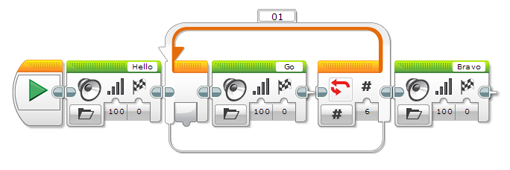
\includegraphics[width=1\columnwidth]{legoLoop.png}
      \caption{Program control flow example in \lego: The robot says ''Hello'' once, then ``Go'' six times, then ``Bravo'' once.}
      \label{fig:legoloopcount}
			\vspace{-.4cm}
   \end{figure}


Multi-threading controls are also found in \trik (\texttt{fork}, \texttt{join}, \texttt{kill thread}), in  \lego for running tasks simultaneously (\texttt{sequence plug exit}) and in \robotmesh, for example in blockly,  \texttt{start block} creates a thread, \texttt{sleep for x seconds} forces a thread to yield. See feature \fmultithread below for more information.

\parhead{\fmodularity.} Despite our environments being user-oriented, the majority (17/29) offers modularization concepts (e.g., functions) to structure larger missions. We found functions, which are graphically represented using dedicated blocks, in the environments called functions or procedures, or modules; each having a name with input parameters and (often) return values. These provide a relatively basic, but pragmatic modularity mechanism, which apparently the non-technical end-users of the environments can utilize.
Examples include \metabot, \ardublockly, \openroberta, \choregraphe, \sphero, \robotmesh, \metabot, \makeblock, \ozoblockly, and \turtlebot; these create mission modules using functions and function calls. \choregraphe implements robot behaviors as boxes, which are connected in a flow chart to form a mission. \lego imports blocks from external environments that are compatible with \lego. \trik implements subprograms, functions, and module with symbolic icon of what these components do; in this way they become mission modules. \picaxe implements procedures of particular concepts, which then can be invoked and used. %\missionlab has predefined states used to build a state machine for a given mission. % -> not sure about the states

%\tivipe is a bit special in this respect, since the underlying platform wraps functions (written in any of the supported languages) with graphical modules, as shown in \figref{fig:tivipe}.
%https://www.tivipe.com/2016/08/30/merging-modules/#more-461

%\begin{figure}[b]
%\vspace{-.4cm}
     %\centering
    %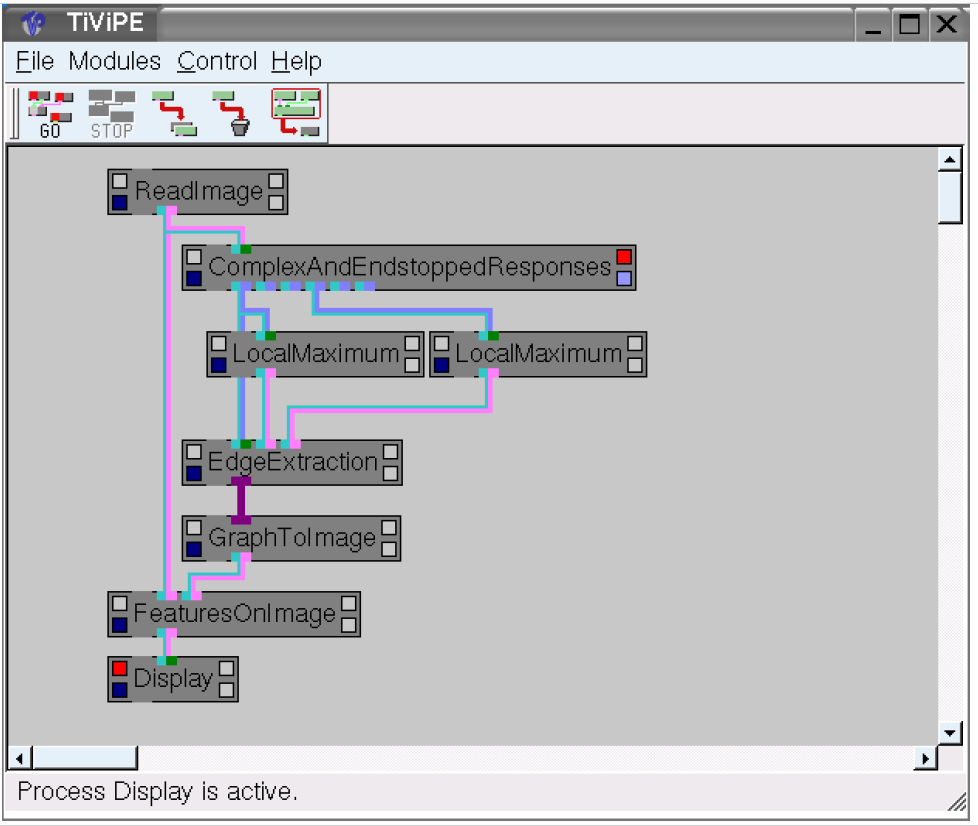
\includegraphics[width=.8\columnwidth]{fig/examples/tivipe.png}
      %\caption{\tivipe's graph-based notation}
      %\label{fig:tivipe}
   %\end{figure}

\parhead{\fdatatypes.} 25 of our environment's main languages offer dedicated data types, such as for variables or functions, comprising primitive and compound types. Only \flyaq, \missionlab, \tivipe, and \trik do not have exclusive variable data types. The primitive types we found include integer, decimal, character, float, number, and Boolean, while compound types include string, arrays, table, and lists. Not surprisingly, we also found domain-specific types, such as sound in \ozoblockly, degrees in \tello, and color in \sphero. The environment \lego calls the Boolean type logic, apparently also for enhancing comprehension by end-users. In \aseba, state is a type, which is essentially an enum (e.g., a variable temperature can take the values off, low, medium or high). %, and light is a variable that can take values like on and off. 

\parhead{\ffunctionlib.} Almost all of the languages come with function libraries that offer typical arithmetic, logic, and string operations on data, but also complex algorithms used to process data. 
% I think 24/29 is wrong; that's why I removed it
%\missionlab, \flyaq, \aseba, \codelab, and \tello do not offer such libraries. % -> aseba should have, please double-check!
Essentially, we found the full range of functions one would expect, including logical operators (e.g., conjunction, disjunction, negation).
%For instance, the logic operations include comparison (e.g., and/or, not, true/false, null, and test.
mathematics functions for trigonometric calculations, rounding, aggregation, and so on. 
%constant, number property, change by x, round, list evaluation, remainder of, constrain, random (integer, fraction), squareroot, return constant(sqrt, pi,...), sum of list, array operations, and range.
String operations include create, append, build string, length, substring; while list operations include find, sublist, isEmpty, join, and so on.  %Math box and data edit box in \choregraphe.     

 
\parhead{\factions} Every language provides statements representing actions. These are activities that robots execute to achieve a given task. Some are reactions to events, while others are activities that are imperatively specified in the mission.

The first distinguishing characteristic we found is the action type. Specifically, actions can be of type:
\begin{itemize}
	\item Instantaneous action, which is executed immediately and only once, such as take photo in \flyaq. %or pause and, resume~\cite{PICAXE}, -> not a good example for instantaneous
	\item Continuous action, which execute immediately for an infinite amount of time or a fixed time, for instance, ``random eyes duration ms" in \openroberta changes the NAO robot's eye colors a for specified duration in milliseconds. Another example is follow line in \lego and \sphero, or record a video in \flyaq.
	\item Delayed action, which starts after a delay.
\end{itemize}

The majority supported is the instantaneous action. The others typically require some notion of time and timer manipulation, where we found different realizations. In \lego the ``get value ms timer'' block is used as a sensor to read the current time for another block, while the ``reset timer'' block is used to reset the internal timer to zero. Similar time constructs also exist in other environment, such as the ``wait time'' and ``elapsed time'' blocks in \ardublockly, the ``set roll time'' in seconds as a variable, ``time elapsed'', ``get current time'', ``set timeout'', ``set time interval'' in \sphero, the ``set timer (seconds)'', ``timer'', ``wait (seconds)'' in \vex.

Then, the environments typically realize concrete actions as dedicated language concepts, which sometimes results in relatively large languages. We classified the actions actuation, communication, and movement actions as follows.

\f{ActuationAction}. This action refers to device/actuator-related activities, such as grasp an object, motor movements, or play audio. More examples include get button code, play tones, sound, stop motors, clear encoder, angular servo, turn on LED, detection with video camera, line detector, video streaming enabling, beep note, buzzer, display, status light, object observation, taping, face status (smile, frown), among others. This illustrates that the languages can become relatively large when (as for most languages) no library mechanism is provided. %lift, backpack, speak, think, change color, hide number, change volume, screen print, screen draw(line/object), start timer, set robot state, say hello, stand-up, wave with hand, move, DoPhoto, monitor street (road task), Intercept Object, LeaveRoom, Localize position, LookForObject, MarkNearestObject, MarkNearestDoor, MoveAhead, MoveAway, MOveForward, MoveToward, PickUp, SurveryRoom, Talk, Terminate, TrackTarget, Wait, Wander, follow line, gripper(open, close, stop), set mode(active, rest, sit). \patrizio{not sure we need all this}\\ 

\f{CommunicationAction}. This action includes interacting with humans or other agents. Communication with humans can be of the form of text, video, or audio. Non-human agents can be categorized as tuple space, publish-subscribe or message passing. Tuple space is a shared space where shared data items are kept for access to entities entitled to access them. In publish-subscribe the publishers create messages regardless of receivers, while subscribers receive messages they have subscribed to.
%
Communication examples include infrared messages exchanged among robots in \edison, \lego, and \openroberta, and Bluetooth messages exchanged between robots in \lego. In \missionlab, robots can share information about target goal position and map of the environment among each other directly or through broadcasts. \sphero, \vex, \makeblock, and \tello broadcast message between robots. \flyaq supports synchronization and communication messaging among drones at run time.  \trik supports sending message to other robots. For what concerns human and central system to robot communications, examples are hand-clap and touch in \aseba, and \enchanting, send text, send number, send command, receive character, send character, send, and receive message in \tello, speak short phrase in \codelab, say text in \trik, \tivipe from the robot to the environment. In \choregraphe robot can share text with humans. In \arcbotics, humans interact with robot through beep, status led colors, infrared remote code and \picaxe communicates through infrared messages. Eleven of the 29 environments do not offer any communication language constructs.
	
\f{MovementAction}. This kind of action manages the mobility of robots. Languages offer concepts that specify how a robot moves from one location to another. Such  concepts are either absolute ``map coordinates,'' or relative, like direction, distance or travel time.

Few of the environments support absolute movement actions, such as goto (coordinates) in \flyaq, \missionlab, and \makeblock; moveto (coordinates), movefast (coordinates, duration) in \tivipe; roll (angle, speed, time), spin(angle, time in seconds) in \sphero; drive (distance) in \codelab. For relative movements we mention go/move/drive/turn/fly (forward/backward/left/right/room) as seen in most of the environments. % , such \metabot, \trik, and \lego.





%\parheadit{Actuation examples identified} - 

 
%\parheadit{Action type examples}


%\parheadit{Communication examples} 

%\parheadit{Movement examples} 

\parhead{\fevents}. 24 or our languages provide event support, which concerns language abilities to handle events like creating event handlers, the types of events that can be recognized, and mechanisms of synchronizing events to subsequent actions. The common language constructs for event support identified include when (event), when (event) do, wait for (event), wait until (event), wait (event), on (event), capture(event), move until (event), broadcast and wait (event) in \vex. \missionlab has even more domain-specific events, such as AtGoal or AtEndOfHall. 
%and delay (event).
The events are sensory data that trigger the next robot action. However, the environments \arcbotics, \tivipe, \minibloq, \turtlebot, and \robotc do not have event support in their languages.

% I don't believe that it's only 26! it should be all!
\parhead{\freadsensor.} All of our languages provide dedicated concepts for reading sensor data. These are used to capture data through sensor readings, to steer the robot's next action. 
%Much as most environments offered language support to capture respective sensor data, \turtlebot and \missionlab do not offer language concepts to manipulate sensors while \choregraphe supports vision recognition using vision reco box and sound recognition using speech reco box. \ozoblockly uses proximity sensor concept to detect objects without details of the sensor.\\
Common sensors captured through the concepts  include gyro for measuring rotations, light/light intensity, sound/clap detector, touch, temperature/thermometer, ultrasonic for measuring distance, timer, compass, accelerometer, gesture detector, and face recognizer. Other sensors are sonar, infrared ranger, GPS module, finger print scanner, energy meter, line detector, and so on. Each of which is typically realized as a dedicated concept in the language.

%, angle reader, line tracker, potentiometer, velocity, power(wats), current (amps), magnetometer, and force resister. The number of sensors on the robot and nature of the missions the robot is designed for determine the language constructs for the sensors. 

\parhead{\fexceptions.} Only three environments, namely \openroberta, \choregraphe, and \codelab offer support for exception handling, and only in their textual languages (not their primary, visual DSLs). % in their text notation but none in the graphical notation. -> double-check!
More specifically, \openroberta exploits the Python exception handler. \choregraphe exploits the try/catch block for all errors in its C++ software development kit (SDK), and the try/catch block for face detection errorr in its Python SDK. \codelab offers support for exception handling for very specific error (e.g., action error, animations not loaded, can not place objects on this, connection aborted). %, connection check failed, connection error, no devices found, not pickupable, and robot busy.

\parhead{\ffileaccess.} Seven of our visual languages provide concepts for file access. For example, \lego provides blocks for reading and writing data to the local storage, and to close or delete a file. Such files can record, for instance, ambient light measurements taken at given time intervals.
%, which are stored in memory and can be displayed on the LCD display screen ~\cite{LEGO}.
%\trik allows writing to the robot's file system, \choregraphe supports open, close and save operations to file while \missionlab offers read, write, close and delete language construct for file operations. \picaxe also supports read and write operations.
% -> five are given in the text, but you count seven; double-check!
The rest of the environments do not offer any language support for file access operations.

\parhead{\fmultithread} Eight of our languages and environments provide support for concurrency. It allows users to do several activities without waiting for one activity to end, improving the performance of executions.

In \robotmesh, using the Blockly editor,  \textit{start} block creates a thread, \textit{sleep} for x seconds forces the thread to \textit{yield}, \textit{start autonomous} creates a thread that runs the autonomous mode of the robot, and \textit{start driver} creates a thread that runs a driver. Recall that \robotmesh also supports various textual general-purpose languages (cf. \tabref{notation}), where the typical multi-threading concepts can be used. For instance, in Python it is sys.run\_in\_thread(f), sys.thread\_id(), sys.sleep(t). In C++, it is thread (void (*callback)(void)), get\_id(), join(), interrupt(), yield(), sleep\_for(unit32\_t time\_ms), lock(), try\_lock(), unlock(). \trik offers fork, join, kill thread, and send message to thread.

Furthermore, \lego offers dedicated blocks for creating parallel tasks, %, though the simultaneous tasks need to be manually verified to avoid resource conflicts.
as well as \makecode and \robotc.
%\textit{run in parallel} to support multithreading of mission tasks.
\tivipe offers \textit{splitSCIS} to split and run modules in parallel. % -> you said three, but why exactly three?
\missionlab supports Cthread, which is a lightweight process threads package that operates under Unix-style operating systems. Also \picaxe supports multi-tasking with operations such as restart, resume, and suspend.





  %\begin{figure}[h]
% \subsection{How the environments differ}
% \noindent
% General language features ~\cite{Clark}; notation is the concrete syntax of a language expressed either as textual syntax or visual syntax. Abstract syntax describes the vocabulary of the concept and how they are combined, while semantics describes what the language represents and means. Mapping feature describes how the language translates to other languages, its semantic equivalence, abstraction level with respect to similar languages and also internal mapping of the abstract syntax to concrete syntax as part of the language architecture. While extensibility of the language states how the language handles adding new concepts to boost its expressiveness. By considering features as end-user visible characteristics of the system, the environments can be compared based on; notation, extensibility, semantics and some aspects of mapping.
% Feature matrix\\
% $\bullet$ Notation matrix\\
% $\bullet$ coupling and reuse of mission artifacts in different contexts\\
% $\bullet$ control flow at run time; imperative (sequence and branch, in concurrent threads, reactive to events or declarative)\\
% editing features (syntax, semantic 

% What made the environments different\\
% $\bullet$ \parhead{Based on underlying technology} blockly based, scratch based, or generic \\
% $\bullet$ \parhead{Connection of blocks} flow chart based or nonflow chart (no links between blocks)\\
% $\bullet$ \parhead{Closeness of mapping} icon based or regular graphical blocks\\
% $\bullet$ \parhead{User domains} students focused (learning), electro-mechanical domain with features of electronics components like motors, programming domains demonstratting features of programming languages,\\ 
% $\bullet$ \parhead{Semantics} are the languages interpreted or compiled. The common generated code languages including; Java Script, Java, C/C++, Python.\\
% $\bullet$ \parhead{Control flow Vs Data flow based}. Control flow based languages graphical languages organize functional blocks into directed graph using arrows. A current block executes command and passes control to the next block based on the output generated. While in data flow based languages, program blocks are data variables that receive data from sensor system, whose value determines the next course of action ~\cite{Mordvinov2017}.
% ======================
% To be crosschecked~\cite{crosscheck}

% \begin{itemize}
% %In robotics, who specifies the mission requirements? (user domain expert, robotic engineer)
%     \item Task features; behavioral/functional model
%     \item Environmental features
%     \item Performance metrics; governing rules that constrain the behavior of the task
%     \item Robot capabilities; physical parts(actuators) that exhibit the behavior of the task
%     \item Mission goal; user goal, purpose of the mission
%     \item Single robot or team of robots mission, if multi-robots, the task distribution/delegation strategy (automatic or explicitly specified).This also includes interactive missions where humans work with robots.
%     \item In quantitative specifications, execution times for respective tasks should be specified otherwise sequence of specification for qualitative specifications.This can be an input to motion planning unit.
%      \item Text; type or select from drop-down list
%     \item Visual/graphical; point at locations to visit in a map, drag and drop domain primitive icons to define sequence of events.
%     \item Audio interaction with robot
%     \item task specification tree where nodes are declarative specification of tasks to perform\cite{Doherty2013}. Can missions be decomposed to tasks and subtasks to form a task forest or bigger tree? Weintrop et al \cite{Weintrop2018} reports use of trees to hierarchically program tasks. Robot routine is broken  into  a series of steps, with each step having sub steps, resulting into hierarchical program as implemented in universal robots' polyscope interface.
% \end{itemize} 
% \claudio{Can you try to put here for each RQ the concepts that aims at answering that RQ. For example, 
% RQ1: Debugging, Simulator.}
% \claudio{If you collected something that is not mapped to an RQ you have two options:
% 1 - you drop it. Because the information is not useful
% 2 - you add a new RQ.}